\documentclass{../oss-handout}
\usepackage{enumitem}
\usepackage{tikz}
\usepackage{siunitx}
\usepackage{amsmath}
%\usepackage{newtxtext,newtxmath}
\usepackage{cancel}
\usepackage[ISO]{diffcoeff}
\usepackage{circuitikz}

\sisetup{
  inter-unit-product=\cdot,
  per-mode=symbol
}
\tikzset{
  >=latex,
  voltage dir=RP
  }
\tikzstyle{vectors}=[ultra thick,->]

\setlength{\parindent}{0pt}
\setlength{\parskip}{6pt}
\setlength{\headheight}{26pt}

\newcommand{\pic}[2]{\includegraphics[width=#1\textwidth]{#2}}

%%%% Set the page style for the document
\pagestyle{plain}

% Course & handout information
\renewcommand{\institution}{Olympiads School}
\renewcommand{\coursetitle}{AP Physics C}
\renewcommand{\term}{Summer 2022}
\title{Solutions to E\&M Mock Exam}

\begin{document}
\thispagestyle{title}
\gentitle

\begin{enumerate}[leftmargin=17pt]
  \item\textbf{(D)} This problem is best solved using Gauss's law. For a very long (i.e.\ infinitely long),
  uniformly charged rod drawn below,  we can draw a Gaussian surface. At a distance of $r$, the
  electric flux is $\Phi=EA=Eii(2\pi rL)$, while the enclosed charge is $q_\text{encl}=\gamma L$,
  where $\gamma$ is the (uniform) charge density.
%   If the strength of the electric field is $E_1$ at a distance
%  $r_1$ from the axis of the rod, at what distance from the axis is
%  the field strength $E_1/4$?
  \begin{center}
    \pic{.25}{rod1}
  \end{center}
  Equating the two, and solving for the electric field strength, we have:
  \begin{displaymath}
    \Phi = E(2\pi rL) = \frac{\gamma L}{\epsilon_0}
    \quad\rightarrow\quad E = \frac{\gamma}{2\pi r\epsilon_0}
  \end{displaymath}
  The electric field strength scales with 1/r, therefore to decrease the strength by a factor
  of 4 requires an increase in r by a factor of 4 as well.

\item\textbf{(C)} The total flux is equal to $\Phi=\dfrac q{\epsilon_0}$, regardless of where the
Gaussian surface is placed. Therefore, both spherical surface will have the same flux. (The difference
is that the outer surface has a larger area, but also a weaker electric field.)
\begin{center}
   \begin{tikzpicture}[scale=.7]
      \fill circle(.08) node[above]{$+q$}; 
        \draw[thick,dashed] circle(1);
        \draw[thick,dashed] circle(2);
      \end{tikzpicture}
    \end{center}

\item\textbf{(A)} For a point charge, the electric field strength scales with $1/r^2$ which means that
the electric field at the outer surface will be 1/4 the strength.

\item\textbf{(E)} We can do a free-body diagram on sphere $X$. The electrostatic force $F_q$ is repulsive.
\begin{center}
  \begin{tikzpicture}[scale=.7]
    \fill circle(.13);
    \draw[vectors] (0,0)--(0,1.5) node[above]{$T$};
    \draw[vectors] (0,0)--(0,-2) node[below]{$Mg$};
    \draw[vectors] (.1,0)--(.1,.7) node[right]{$F_q$};
  \end{tikzpicture}
\end{center}
Balancing the forces, we have:
\begin{displaymath}
  T+F_q-Mg=0 \quad\rightarrow\quad F=Mg-F_q=\boxed{Mg-\frac{kq^2}{d^2}}
\end{displaymath}
  
  
\item\textbf{(C)} Although it does not look like it, the problem is symmetric. The total
flux through all the surface are the same. Therefore the flux through each surface is
$\Phi/4=\boxed{q/4\epsilon_0}$.
\begin{center}
  \pic{.2}{tetrahedral}
\end{center}


\item\textbf{(D)} As the current begins to flow in the circuit, a voltage is build up in the capacitor.
  The current will decrease exponentially:
  \begin{displaymath}
    I=\frac{\mathcal E}Re^{-\frac t{RC}}
  \end{displaymath}
  \begin{center}
    \begin{tikzpicture}
      \draw[very thick](1.75,.35)--(1.2,0) node[midway,above left]{$S$}
      --(0,0) to[battery1,l=$\mathcal E$] (0,2)
      to[R,l=$R$] (4,2) to[C,l=$C$] (4,0)--(1.8,0);
    \end{tikzpicture}
  \end{center}
  The voltage across the resistor will also decrease exponentially.
  \begin{displaymath}
    V_R=IR = \mathcal Ee^{-\frac t{RC}}
 \end{displaymath}


%%%  \uplevel{\rule{\linewidth}{.5pt}}
%%%
%%%  \uplevel{
%%%    \textbf{Question \ref{rcirc1}--\ref{rcirc2}}
%%%    \cpic{.35}{r-circuit1}
%%%
%%%    \vspace{-.1in}An electric circuit consists of a \SI{12}{\volt} battery, an
%%%    ideal \SI{10}{\ampere} fuse, and three \SI2{\ohm} resistors connected as
%%%    shown above.
%%%    }
\item\textbf{(A)} This is a very simple question. The voltage across $A$ and $C$ must be the same
as the battery.

\item\textbf{(C)} The resistance between $A$ and $C$ is $R_\text{eq}=2+2=\SI4\ohm$. Therefore the current 
  anywhere between $A$ and $C$ would be:
  \begin{displaymath}
    I=\frac VR=\frac{12}4=\boxed{\SI3\ampere}
  \end{displaymath}


\item\textbf{(C)} When the switch is closed, the effective resistance across 1 and 2 (which are in parallel)
would decrease, and the equivalent resistance in the entire circuit decreases. Therefore the 
total current out of the battery increase, and we would see that bulb 3 increase in brightness. However,
since current is split between 1 and 2, bulb 2 would decrease in brightness.

\item\textbf{(E)} When the wire is then cut in half and the two halves are connected in parallel, the length decreases
by a factor of 1/2, while the cross sectional area increase by a factor of 2.
Therefore the new resistance decreases by a factor of 1/4:
\begin{displaymath}
  R=\frac{\rho L}A\quad\quad R'=\frac{\rho(L/2)}{2A}=\frac14R
\end{displaymath}
When connected across the same battery, the current would increase by a factor of 4. And since the voltage
across the resistor does not change, the power dissipated also increases by a factor of 4:
\begin{displaymath}
  P=\frac{V^2}R  \quad\quad P'=\frac{V^2}{R/4}=4P
\end{displaymath}

\item\textbf{(D)} After the switch has ben closed for a long time, the voltage across the capcitor is the same as the battery,
i.e.\ $V_c=\mathcal E$. The energy stored in the capacitor is:
\begin{displaymath}
U_c = \frac12CV_C^2=\frac12C\mathcal E^2=\frac12(\num{10e-6})(10)^2=\num{5.0e-4}=\boxed{\SI{500}{\micro\joule}}
\end{displaymath}


\item\textbf{(C)} In the diagram, the magnetic field points into the page, by the convention of the notation. When
the electron enters the magnetic field, it will experience an upward magnetic force that puts it into
circular motion. Therefore the motion is circular and clockwise.
  \begin{center}
    \begin{tikzpicture}[scale=.9]
      \foreach \x in {0,...,5}{
        \foreach \y in {0,...,3} \node at (\x,\y){$\times$};
      }
      \draw[dashed] (-.3,-.3) rectangle(5.3,3.3);
      \node at (1.4,2.2){$\vec B$};
      \draw[vectors] (6.3,1.5)--(5.3,1.5)node[pos=0,right]{$e^-$};
    \end{tikzpicture}
  \end{center}

\item\textbf{(B)} The magnetic field that is produced by the current $I$ points into the page at $P$.
The magnetic field generated by the current $2I$ points out of the page, but with a larger
magnitude. Therefore the total magneitic field piounts out of the page.
%%%  \uplevel{
%%%    \rule{\linewidth}{.5pt}
%%%    \textbf{Questions \ref{contour1}--\ref{contour2}}
%%%    \cpic{.37}{contours}
%%%    A fixed charge distribution produces the equipotential lines shown in the
%%%    figure above.
%%%  }

\item Which of the following expressions best represents the magnitude of
  the electric field at point $P$?
%%%  \label{contour1}
%%%  \begin{choices}
%%%    \choice $\dfrac{\SI{10}{\volt}}{\SI{.14}{\metre}}$
%%%    \choice $\dfrac{\SI{10}{\volt}}{\SI{.04}{\metre}}$
%%%    \choice $\dfrac{\SI{25}{\volt}}{\SI{.14}{\metre}}$
%%%    \choice $\dfrac{\SI{25}{\volt}}{\SI{.04}{\metre}}$
%%%    \choice $\dfrac{\SI{40}{\volt}}{\SI{.25}{\metre}}$
%%%  \end{choices}

\item\textbf{(A)} The direction of the electric field points from high to low potential, and perpendicular
to the equipotential contours. At $P$,this means that $\vec E$ points to the left.

\item The gain in kinetic energy for bothquestion A helium nucleus (charge $+2q$ and mass $4m$) and a lithium nucleus
%%%  (charge $+3q$ and mass $7m$) are accelerated through the same electric
%%%  potential difference, $V_0$. What is the ratio of their resultant
%%%  kinetic energies, $\dfrac{K_\text{Li}}{K_\text{He}}$?
%%%  \begin{choices}
%%%    \choice$\dfrac23$
%%%    \choice$\dfrac67$
%%%    \choice 1
%%%    \choice$\dfrac76$
%%%    \choice$\dfrac32$
%%%  \end{choices}
%%%  \uplevel{ \rule{\linewidth}{.5pt}}
%%%  
%%%  \question The electric potential in the $xy$-plane in a certain region of
%%%  space is given by $V(x,y)=6x^2y-2y^3$, where $x$ and $y$ are in meters and
%%%  $V$ is in volts. What is the magnitude of the $y$-component of the electric
%%%  field at the point $(-1,2)$?
%%%  \begin{choices}
%%%    \choice\SI{0}{\volt\per\metre}
%%%    \choice\SI{4}{\volt\per\metre}
%%%    \choice\SI{18}{\volt\per\metre}
%%%    \choice\SI{24}{\volt\per\metre}
%%%    \choice\SI{30}{\volt\per\metre}
%%%  \end{choices}
%%%
%%%  \uplevel{ \rule{\linewidth}{.5pt}}
%%%  
%%%  \uplevel{
%%%    \centering
%%%    \begin{tikzpicture}
%%%      \draw[thick](-4,0) circle(.2) node{$\bm +$};
%%%      \draw[thick] circle(.2) node{$\bm -$};
%%%      \draw[thick]( 4,0) circle(.2) node{$\bm +$};
%%%      \draw[thick,<->](-3.8,0)--(-.2,0) node[midway,fill=white]{$a$};
%%%      \draw[thick,<->]( 3.8,0)--( .2,0) node[midway,fill=white]{$a$};
%%%      \node[below] at (-4,-.2){Proton};
%%%      \node[below] at ( 0,-.2){Electron};
%%%      \node[below] at ( 4,-.2){Proton};
%%%    \end{tikzpicture}
%%%  }
%%%
%%%  \question Two protons and an electron are assembled along a line, as shown
%%%  below. The distance between the electron and each proton is $a$. What is the
%%%  work done by an external force in assembling this configuration of charges?
%%%  \begin{choices}
%%%    \choice $-2\dfrac{ke^2}a$
%%%    \choice $-\dfrac32\dfrac{ke^2}a$
%%%    \choice $\dfrac12\dfrac{ke^2}a$
%%%    \choice $\dfrac32\dfrac{ke^2}a$
%%%    \choice $3\dfrac{ke^2}a$
%%%  \end{choices}
%%%
%%%  \uplevel{
%%%    \rule{\linewidth}{.5pt}
%%%    \textbf{Questions \ref{rain1}--\ref{rain2}}
%%%
%%%    A cloud contains spherical drops of water of radius $R$ and charge $Q$.
%%%    Assume the drops are far apart.
%%%  }
%%%
%%%  \question The electric field $E_0$ and potential $V_0$ at the surface of each
%%%  drop is given by which of the following?
%%%  \label{rain1}
%%%  
%%%  \begin{tabular}{ccc}
%%%    & $E_0$ & $V_0$ \\ \hline
%%%    (A) & 0 & 0 \\
%%%    (B) & $\dfrac{kQ}R$ & $\dfrac{kQ}{R^2}$ \\
%%%    (C) & $\dfrac{kQ}{R^2}$ & $\dfrac{kQ}R$ \\
%%%    (D) & 0 & $\dfrac{kQ}R$ \\
%%%    (E) & $\dfrac{kQ}R$ & 0
%%%  \end{tabular}
%%%
%%%  \question If two droplets happen to combine into a single larger droplet, the
%%%  new potential $V$ at the surface of the larger droplet is most nearly equal to
%%%  \label{rain2}
%%%  \begin{choices}
%%%    \choice $3V_0$
%%%    \choice $2V_0$
%%%    \choice $\dfrac2{2^{1/3}}V_0$
%%%    \choice $2^{1/3}V_0$
%%%    \choice $V_0$
%%%  \end{choices}
%%%  
%%%%  \question A point charge $-Q$ is located at the origin, while a second point
%%%%  charge $+2Q$ is located at $x=d$ on the $x$-axis, as shown above. A point on
%%%%  the $x$-axis where the net electric field is zero is located in which of the
%%%%  following regions?
%%%%
%%%%  \vspace{.1in}
%%%%  \begin{minipage}{.3\linewidth}
%%%%    \begin{tikzpicture}
%%%%      \draw[very thick,->](-1,0)--(3,0) node[right]{$x$};
%%%%      \draw(0,.1)--(0,-.1) node[below]{0};
%%%%      \draw(1,.1)--(1,-.1) node[below]{$\dfrac{d}2$};
%%%%      \draw(2,.1)--(2,-.1) node[below]{$d$};
%%%%      \fill circle(.05) node[above]{$-Q$};
%%%%      \fill(2,0) circle(.05) node[above]{$+2Q$};
%%%%    \end{tikzpicture}
%%%%  \end{minipage}
%%%%  \begin{minipage}{.4\textwidth}
%%%%    \begin{choices}
%%%%      \choice $-\infty<x<0$
%%%%      \choice $0<x<\dfrac{d}2$
%%%%      \choice $\dfrac{d}2<x<d$
%%%%      \choice $d<x<\infty$
%%%%      \choice No region on the $x$-axis
%%%%    \end{choices}
%%%%  \end{minipage}
%%%%  
%%%  \uplevel{ \rule{\linewidth}{.5pt}}
%%%  
%%%  \question An inductor of inductance $L$ is connected in series with a
%%%  resistor of resistance $R$, a battery of emf $\mathcal E$, and a switch, as
%%%  shown above. When the switch is closed, the current $I$ in the circuit
%%%  increases with time, approaching the value $I_\text{max}$. What is
%%%  $I_\text{max}$?
%%%  
%%%  \begin{minipage}{.4\textwidth}
%%%    \begin{tikzpicture}[scale=1.2]
%%%      \draw[thick](2.3,2) to[short,*-](4,2) to[R,l=$R$](4,0) to[L,l=$L$](0,0)
%%%      to[battery1,l=$\mathcal E$] (0,2) to[short,-*](1.7,2)--(2.3,2.2);
%%%    \end{tikzpicture}
%%%  \end{minipage}
%%%  \begin{minipage}{.4\linewidth}
%%%    \begin{choices}
%%%      \choice $R/L\mathcal E$
%%%      \choice $RL/\mathcal E$
%%%      \choice $\mathcal E/RL$
%%%      \choice $\mathcal E/R$
%%%      \choice $L\mathcal E$
%%%    \end{choices}
%%%  \end{minipage}
%%%  \newpage  
%%%  
%%%  \uplevel{
%%%    \textbf{Questions \ref{emf1}--\ref{emf2}}
%%%    
%%%    An emf of \SI{20}{\volt} is induced around a metal ring by increasing a
%%%    uniform magnetic field at a constant rate from zero to a final magnitude
%%%    of \SI{1.0e-2}{\tesla} throughout the region enclosed by the ring. The field
%%%    direction is perpendicular to the plane of the ring.
%%%  }
%%%  
%%%  \question If the area enclosed by the ring is \SI{4.0e-3}{\metre\squared},
%%%  what is the time interval during which the field is increased?
%%%  \label{emf1}
%%%  \begin{choices}
%%%    \choice \SI{2.}{\micro\second}
%%%    \choice \SI{5.}{\micro\second}
%%%    \choice \SI{10}{\micro\second}
%%%    \choice \SI{20}{\micro\second}
%%%    \choice \SI{50}{\micro\second}
%%%  \end{choices}
%%%
%%%  \question If the electrical resistance of the ring is \SI{500}\ohm, what is
%%%  the rate at which energy is dissipated in the ring as the field is increased?
%%%  \label{emf2}
%%%  \begin{choices}
%%%    \choice\SI{.040}\watt
%%%    \choice\SI{.80}\watt
%%%    \choice\SI{1.25}\watt
%%%    \choice\SI{25}\watt
%%%    \choice\SI{1.e4}\watt
%%%  \end{choices}
%%%
%%%  \uplevel{
%%%    \centering
%%%    \rule{\linewidth}{.5pt}
%%%    \begin{tikzpicture}[scale=.77]
%%%      \draw[dashed,thick,->](-4,0)--(4,0)node[right]{$x$};
%%%      \draw[dashed,thick,->](0,-3)--(0,3)node[above]{$y$};
%%%      \draw[ultra thick](-1,-3)--(-1,3);
%%%      \draw[ultra thick]( 1,-3)--( 1,3);
%%%      \draw[<->](-1,.7)--(0,.7)  node[midway,fill=white]{\small$r$};
%%%      \draw[<->](1,-.7)--(0,-.7) node[midway,fill=white]{\small$r$};
%%%      \draw[ultra thick,->](-1,0)--(-1,1.5) node[left]{$I$};
%%%      \draw[ultra thick,->](1,0)--(1,-1.5) node[right]{$I$};
%%%      \fill circle(.07) node[below left]{$O$};
%%%    \end{tikzpicture}
%%%    \hspace{.3in}
%%%    \begin{tikzpicture}[scale=.77]
%%%      \draw[dashed,thick,->](-4,0)--(4,0)node[right]{$x$};
%%%      \draw[dashed,thick,->](0,-3)--(0,3)node[above]{$y$};
%%%      \draw[ultra thick](-4,0)--(-1,0)--(-1,3);
%%%      \draw[ultra thick](3.8,0)--(1,0)--(1,-3);
%%%      \draw[<->](-1,.7)--(0,.7)  node[midway,fill=white]{\small$r$};
%%%      \draw[<->](1,-.7)--(0,-.7) node[midway,fill=white]{\small$r$};
%%%      \draw[ultra thick,->](-1,0)--(-1,1.5) node[left]{$I$};
%%%      \draw[ultra thick,->](-3,0)--(-2.3,0);
%%%      \draw[ultra thick,->](1,0)--(1,-1.5) node[right]{$I$};
%%%      \draw[ultra thick,->](3,0)--(2.3,0);
%%%      \fill circle(.07) node[below left]{$O$};
%%%    \end{tikzpicture}
%%%  }
%%%
%%%  \question Two long, straight wires are parallel to and equidistant from the
%%%  $y$-axis, as shown above left. Each carries current $I$ in opposite
%%%  directions, resulting in a magnetic field of magnitude $B_0$ at the origin.
%%%  If the wires are each bent into right angles and placed as shown above right,
%%%  what is the magnitude of the magnetic field $B$ at the origin?
%%%  \begin{choices}
%%%    \choice Zero
%%%    \choice Between zero and $B_0/2$
%%%    \choice $B_0/2$
%%%    \choice Between $B_0/2$ and $B_0$
%%%    \choice $B_0$
%%%    \end{choices}
%%%
%%%  \uplevel{
%%%    \centering
%%%    \rule{\linewidth}{.5pt}
%%%
%%%    \begin{tikzpicture}[scale=.8]
%%%      \begin{scope}[rotate=20,very thick,->]
%%%        \draw(-1.5,0) arc(180:-200:1.5);
%%%        \draw(-1.3,0) arc(180:-200:1.5);
%%%        \draw(-1.1,0) arc(180:-200:1.5);
%%%      \end{scope}
%%%      \node at (-2,0) {$I$};
%%%      \node at (0,-3) {Loop $X$};
%%%    \end{tikzpicture}
%%%    \hspace{.3in}
%%%    \begin{tikzpicture}
%%%      \draw[very thick,->](-2.2,0) arc(180:-200:2.2) node[above left]{$I$};
%%%      \node at (0,-3) {Loop $Y$};
%%%    \end{tikzpicture}
%%%  }
%%%
%%%  \question A length of wire carrying a steady clockwise current $I$ is bent
%%%  to form the triple circular loop $X$ above. An identical length of the same
%%%  wire is bent less tightly to form the single loop $Y$ of larger radius, which
%%%  carries the same current $I$. The ratio of the magnetic field strength at the
%%%  center of loop $Y$ to the magnetic field strength at the center of loop $X$ is
%%%  \begin{choices}
%%%    \choice $1/9$
%%%    \choice $1/3$
%%%    \choice 1
%%%    \choice 3
%%%    \choice 9
%%%  \end{choices}
%%%  %\newpage
%%%  
%%%  \uplevel{
%%%	\rule{\linewidth}{.5pt}
%%%    \cpic{.23}{cable-xsection}
%%%  }
%%%  \question The diagram above shows the cross section of a long cable that has
%%%  an inner wire of radius $R$ surrounded by a conducting sheath of outer radius
%%%  $2R$. The wire and the sheath carry currents in opposite directions but with
%%%  the same uniform current density $J$. What is the magnitude of the magnetic
%%%  field at the surface of the outer conductor?
%%%  \begin{choices}
%%%    \choice Zero
%%%    \choice $\dfrac14\mu_0RJ$
%%%    \choice $\dfrac12\mu_0RJ$
%%%    \choice $\dfrac34\mu_0RJ$
%%%    \choice $\mu_0RJ$
%%%  \end{choices}
%%%
%%%  \uplevel{
%%%    %\rule{\linewidth}{.5pt}
%%%    \cpic{.2}{long-wire1}
%%%  }
%%%  \question A long wire of radius $R$ carries a current $I$, as
%%%  shown above, with a current density $J=ar$ that increases linearly with the
%%%  distance $r$ from the center of the wire. Which of the following graphs best
%%%  represents the magnitude of the magnetic field $B$ as a function $r$?
%%%
%%%  \begin{oneparchoices}
%%%    \choice
%%%    \begin{tikzpicture}[scale=1.1]
%%%      \draw[->](0,0)--(2,0)  node[right]{$r$};
%%%      \draw[->](0,0)--(0,1.7)node[right]{$B$};
%%%      \draw[dashed](1,1)--(1,0) node[below]{$R$};
%%%      \draw[ultra thick](0,1)--(1,1);
%%%      \draw[ultra thick,domain=1:1.7] plot(\x,{2.72*exp(-\x)});
%%%    \end{tikzpicture}
%%%
%%%    \choice
%%%    \begin{tikzpicture}[scale=1.1]
%%%      \draw[->](0,0)--(2,0)  node[right]{$r$};
%%%      \draw[->](0,0)--(0,1.7)node[right]{$B$};
%%%      \draw[dashed](1,1)--(1,0) node[below]{$R$};
%%%      \draw[ultra thick](0,0)--(1,1);
%%%      \draw[ultra thick,domain=1:1.7] plot(\x,{2.72*exp(-\x)});
%%%    \end{tikzpicture}
%%%
%%%    \choice
%%%    \begin{tikzpicture}[scale=1.1]
%%%      \draw[->](0,0)--(2,0)  node[right]{$r$};
%%%      \draw[->](0,0)--(0,1.7)node[right]{$B$};
%%%      \draw[dashed](1,1)--(1,0) node[below]{$R$};
%%%      \draw[ultra thick,domain=0:1]   plot(\x,{\x*\x)});
%%%      \draw[ultra thick,domain=1:1.7] plot(\x,{2.72*exp(-\x)});
%%%    \end{tikzpicture}
%%%
%%%    \choice
%%%    \begin{tikzpicture}[scale=1.1]
%%%      \draw[->](0,0)--(2,0)  node[right]{$r$};
%%%      \draw[->](0,0)--(0,1.7)node[right]{$B$};
%%%      \draw[dashed](1,1)--(1,0) node[below]{$R$};
%%%      \draw[ultra thick](0,0)--(1,0);
%%%      \draw[ultra thick,domain=1:1.7] plot(\x,{2.72*exp(-\x)});
%%%    \end{tikzpicture}
%%%
%%%    \choice
%%%    \begin{tikzpicture}[scale=1.1]
%%%      \draw[->](0,0)--(2,0)  node[right]{$r$};
%%%      \draw[->](0,0)--(0,1.7)node[right]{$B$};
%%%      \draw[dashed](1,1)--(1,0) node[below]{$R$};
%%%      \draw[ultra thick] (0,0)--(1,1);
%%%      \draw[ultra thick] (1,0)--(1.7,0);
%%%    \end{tikzpicture}    
%%%  \end{oneparchoices}
%%%  \vspace{.3in}
%%%
%%%  \uplevel{
%%%    \centering
%%%    \rule{\linewidth}{.5pt}
%%%    \pic{.23}{rc-loop}
%%%  }
%%%  \question In the circuit drawn above, the switch $S$ is initially open, and
%%%  the capacitor $C$ is charged with the polarity indicated. The switch is then
%%%  closed, and the capacitor begins discharging through the resistor. Which of
%%%  the following is true of the current that is subsequently induced in the
%%%  circular wire loop near the long, straight wire $AB$?
%%%
%%%  \begin{choices}
%%%    \choice It is counterclockwise and constant.
%%%    \choice It is counterclockwise and increases with time.
%%%    \choice It is counterclockwise and decreases with time.
%%%    \choice It is clockwise and increases with time.
%%%    \choice It is clockwise and decreases with time
%%%  \end{choices}
%%%  
%%%  \uplevel{\rule{\linewidth}{.5pt}}
%%%  
%%%  \question Which of the following statements contradicts one of Maxwell's
%%%  equations?
%%%  \begin{choices}
%%%    \choice A changing magnetic field produces an electric field.
%%%    \choice A changing electric field produces a magnetic field.
%%%    \choice The net magnetic flux through a closed surface depends on the
%%%    current inside.
%%%    \choice The net electric flux through a closed surface depends on the
%%%    charge inside.
%%%    \choice The electric field due to an isolated stationary point charge is
%%%    inversely proportional to the square of the distance from the charge.
%%%  \end{choices}
%%%  \vspace{.7in}
%%%  %\newpage
%%%  
%%%  \uplevel{
%%%    \rule{\linewidth}{.5pt}
%%%  }
%%%  \question A student building a circuit wishes to increase the frequency of an
%%%  oscillator consisting of a capacitor of capacitance $C$ and an inductor of
%%%  inductance $L$. Which of the following would accomplish this objective?
%%%  \begin{enumerate}[nosep,label={\Roman*.}]
%%%  \item Increase $L$
%%%  \item Increase $C$
%%%  \item Decrease $L$
%%%  \item Decrease $C$
%%%  \end{enumerate}
%%%  \vspace{.2in}
%%%  \begin{choices}
%%%    \choice I only
%%%    \choice I or II
%%%    \choice I or IV
%%%    \choice II or III
%%%    \choice III or IV
%%%  \end{choices}
\end{enumerate}
\end{document}
